The radiation pattern is obtained by projecting the received signal onto the target steering 
vector. Suppose the incidence angle of the desired signal is $\phi_0$, the attenuation at angle 
$\phi$ is
\begin{equation*}
    \text{P}\left(\phi\right) = \left|e_r^{H}(\Omega) \cdot e_r(\Omega_0)\right|
\end{equation*}
where $\Omega = \cos\left(\phi\right)$ and $\Omega_0 = \cos\left(\phi_0\right)$.
The radiation patterns are shown below:
\begin{figure}[H]
    \centering
    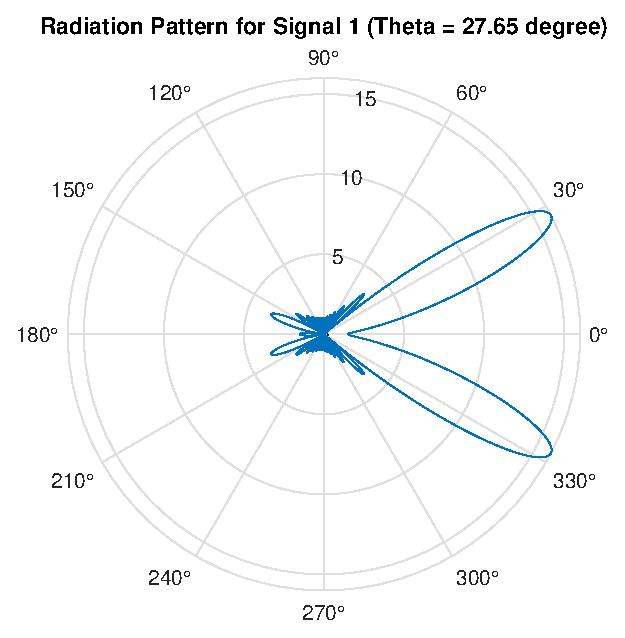
\includegraphics[scale = 0.7]{s1.eps}
\end{figure}
\begin{figure}[H]
    \centering
    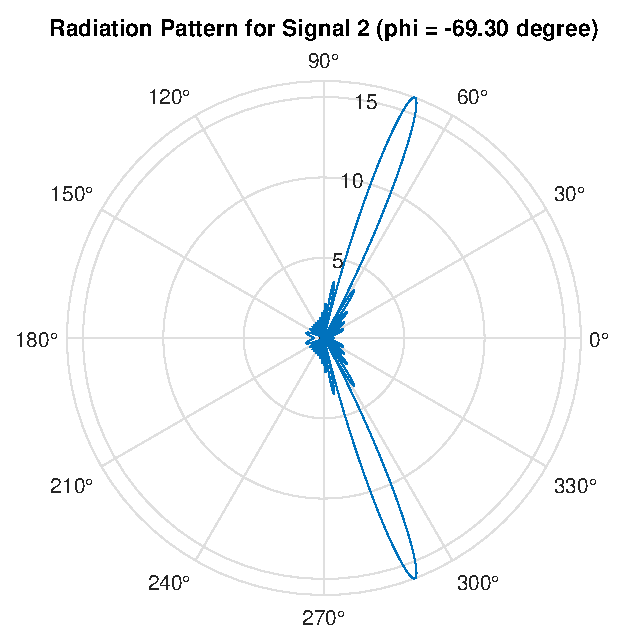
\includegraphics[scale = 0.7]{s2.eps}
\end{figure}
\begin{figure}[H]
    \centering
    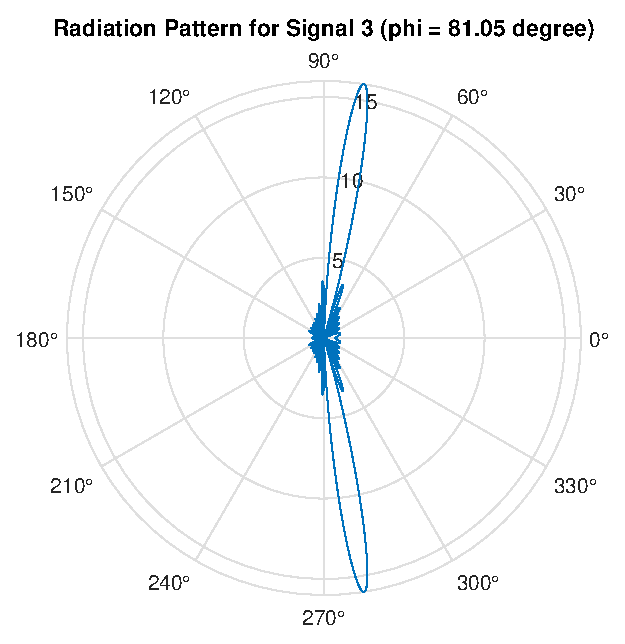
\includegraphics[scale = 0.7]{s3.eps}
\end{figure}
\begin{figure}[H]
    \centering
    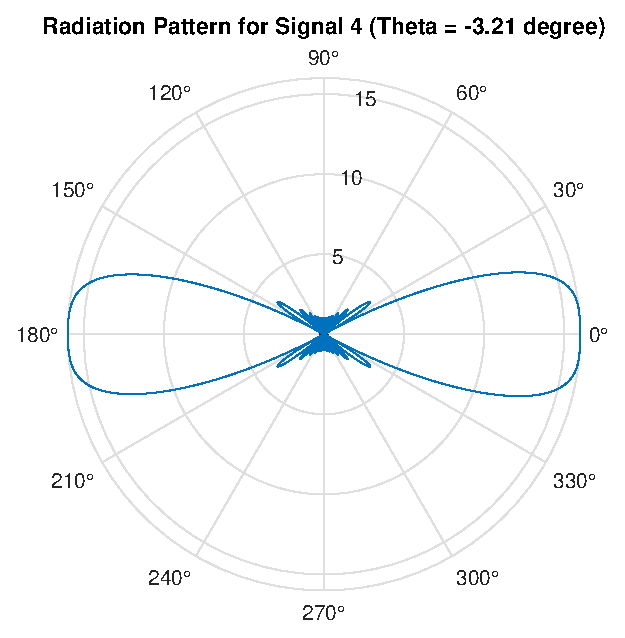
\includegraphics[scale = 0.7]{s4.eps}
\end{figure}
\begin{figure}[H]
    \centering
    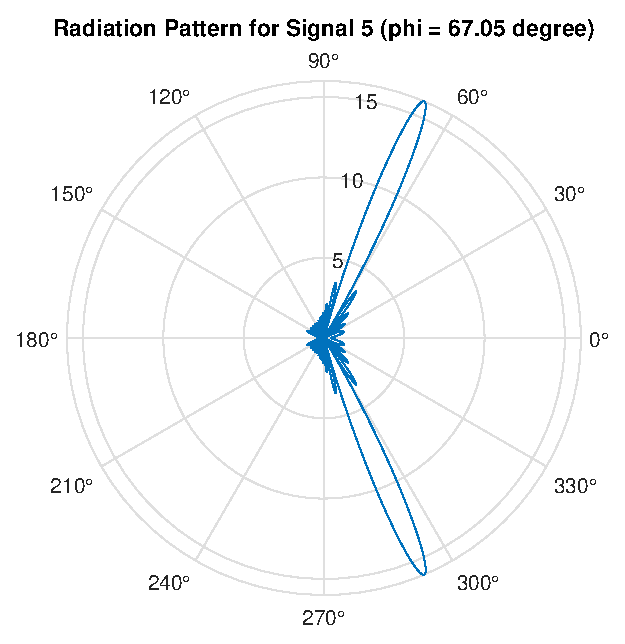
\includegraphics[scale = 0.7]{s5.eps}
\end{figure}
It can be observed that with receive beamforming, the main lobe is aligned with the incidence angle.